\documentclass[unicode,11pt,a4paper,oneside,numbers=endperiod,openany]{scrartcl}

% Required package
\usepackage{amssymb}
\usepackage{graphicx}
\usepackage{amsmath}
\usepackage{matlab-prettifier}
\usepackage{float}
\usepackage[export]{adjustbox}
\usepackage{multirow}
\usepackage{booktabs}
\usepackage{amsthm} % math theorems
\usepackage{ifthen}

\renewcommand{\thesubsection}{\arabic{subsection}}

% 1: command name, 2: Title, 3: subtitle, 4: label, 5: content
\newcommand{\mytheorem}[5]{\newtheorem*{#1}{#2} \begin{#1}[#3]\label{#4} #5 \end{#1}}

% 1: if numbered equation, 2: label, 3: content
\newcommand{\myex}[3]{
    \ifthenelse{\equal{#1}{true}}{
        \begin{equation} \label{#2} \begin{aligned} #3 \end{aligned} \end{equation}
    }{
        \begin{equation*} \label{#2} \begin{aligned} #3 \end{aligned} \end{equation*}
    }
}

% vector shortcut
\newcommand{\myvec}[1]{\begin{bmatrix} #1 \end{bmatrix}}
\newcommand{\myFigureEnergy}[3]{
    \begin{figure}[htbp]
    \centering
    \caption{#1}
    \label{#2}
    \includegraphics[width=\paperwidth, trim={9cm 0cm -2cm 0cm}]{./figures/#3}
    \end{figure}
}
\newcommand{\myFigureComparison}[4]{
    \begin{figure}[htbp]
    \centering
    \caption{#1}
    \label{#2}
    \includegraphics[width=.2\paperwidth, trim={8.5cm 0cm 0.5cm 0cm}]{./figures/#3}
    \includegraphics[width=.2\paperwidth, trim={0.5cm 0cm 8.5cm 0cm}]{./figures/#4}
    \end{figure}
}

\input{assignment.sty}
\begin{document}


\setassignment
\setduedate{Wednesday, 8 May 2024}

\serieheader
{Optimization Methods}
{2024}
{\textbf{Student:} Jeferson Morales Mariciano \\\\}
{\textbf{Discussed with:}}
{In-Class Exercise}{}
\newline

%\assignmentpolicy


% EXERCISE 2 %%%%%%%%%%%%%%%%%%%%%%%%%%%%%%%%%%%%%%%%%%%%%%%%%%%%%%%%%%%%%%%%%%%%%%%%%%%%%%%%%%%%%%
\subsection*{2.}
Solve $\min_{x} f(x, y)$ by using both the implemented methods. \\\newline

Matlab scripts are provided in \textit{/code} folder. 
The 3 main files to run are: main.m, cauchyPoint.m, dogleg.m. 
They handle both computations and visualization of the Rosenbrock's function 
with the corresponding trust region methods.

% EXERCISE 3 %%%%%%%%%%%%%%%%%%%%%%%%%%%%%%%%%%%%%%%%%%%%%%%%%%%%%%%%%%%%%%%%%%%%%%%%%%%%%%%%%%%%%%
\subsection*{3.}
Plot the obtained steps on the energy landscape and compare performance of the methods. \\\newline

Hereby the example of the Rosenbrock function has the same parameters as assignment 2:
$tol = 1e-6$, $maxIter = 50000$, $x_0 = \myvec{0 \\ 0}$.
For Trust Region methods, the parameters chosen were:
$\hat{\Delta} = 2$, $\Delta = 0.75$, $\eta = \frac{1}{4}$.

Clearly, the Dogleg method converges faster than the Cauchy Point method.
The convergence plots in Figure \ref{ex1-cauchy-convergence} and \ref{ex1-dogleg-convergence}
show that the Dogleg method converges in 16 iterations, 
while the Cauchy Point method converges in 13972 iterations.
That is due to the fact that the Dogleg method is faster in terms of iterations
because it uses second order information from the hessian.
The Cauchy Point method is faster in terms of time per iteration 
because it is computationally inexpensive:
no matrix factorization are required to compute the step $p_k^C$.
An evaluation of whether an approximate solution for the trust region problem is acceptable
is necessary before employing the Cauchy Point method.



\myFigureEnergy{Cauchy Point method, $x_0 = \myvec{0 \\ 0}$}{ex1-cauchy-energy}{ex1-cauchy-energy.eps}
\begin{figure}[htbp]
\centering
\caption{Cauchy Point method convergence, $x_0 = \myvec{0 \\ 0}$}
\label{ex1-cauchy-convergence}
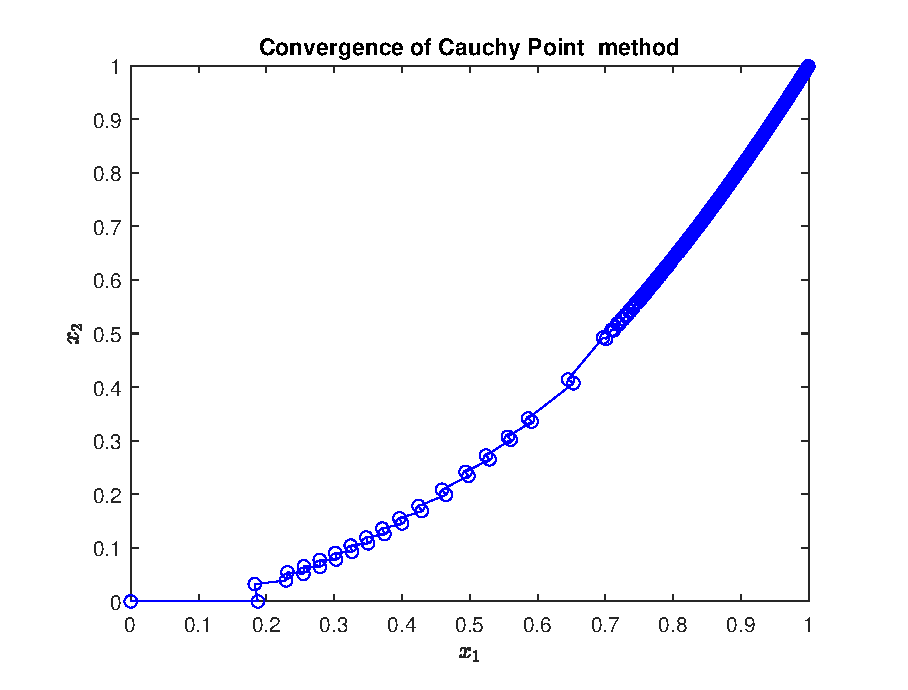
\includegraphics[width=\textwidth, trim={0cm 0cm 0cm 0cm}]{./figures/ex1-cauchy-convergence.eps}
\end{figure}


\myFigureEnergy{Dogleg method, $x_0 = \myvec{0 \\ 0}$}{ex1-dogleg-energy}{ex1-dogleg-energy.eps}
\begin{figure}[htbp]
\centering
\caption{Dogleg method convergence, $x_0 = \myvec{0 \\ 0}$}
\label{ex1-dogleg-convergence}
\includegraphics[width=\textwidth, trim={0cm 0cm 0cm 0cm}]{./figures/ex1-dogleg-convergence.eps}
\end{figure}

% EXERCISE 4 %%%%%%%%%%%%%%%%%%%%%%%%%%%%%%%%%%%%%%%%%%%%%%%%%%%%%%%%%%%%%%%%%%%%%%%%%%%%%%%%%%%%%%
\subsection*{4.}
Compare performance of the trust region method based on Dogleg and on Cauchy point for three
different $x_0$.

\subsubsection*{$x_0 = \myvec{0 \\ 0}$}
Cauchy point method for Figures \ref{ex1-cauchy-energy}, \ref{ex1-cauchy-convergence}.
Dogleg method for Figures \ref{ex1-dogleg-energy}, \ref{ex1-dogleg-convergence}.

\subsubsection*{$x_0 = \myvec{1 \\ 0}$}
Cauchy point method for Figures \ref{ex1-4-10-cauchy-energy}, \ref{ex1-4-10-cauchy-convergence}.
Dogleg method for Figures \ref{ex1-dogleg-energy}, \ref{ex1-dogleg-convergence}.

\myFigureEnergy{Cauchy Point method, $x_0 = \myvec{1 \\ 0}$}{ex1-4-10-cauchy-energy}{ex1-4-10-energy.eps}
\begin{figure}[htbp]
\centering
\caption{Cauchy Point method convergence, $x_0 = \myvec{1 \\ 0}$}
\label{ex1-4-10-cauchy-convergence}
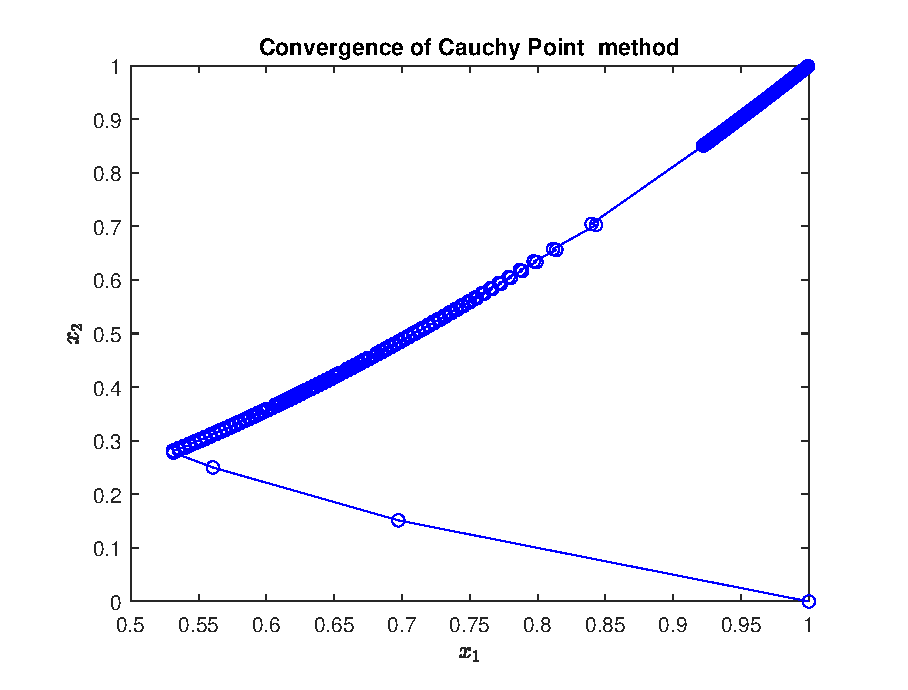
\includegraphics[width=\textwidth, trim={0cm 0cm 0cm 0cm}]{./figures/ex1-4-10-convergence.eps}
\end{figure}


\myFigureEnergy{Dogleg method, $x_0 = \myvec{1 \\ 0}$}{ex1-4-10-dogleg-energy}{ex1-4-10-dogleg-energy.eps}
\begin{figure}[htbp]
\centering
\caption{Dogleg method convergence, $x_0 = \myvec{1 \\ 0}$}
\label{ex1-4-10-dogleg-convergence}
\includegraphics[width=\textwidth, trim={0cm 0cm 0cm 0cm}]{./figures/ex1-4-10-dogleg-convergence.eps}
\end{figure}

\subsubsection*{$x_0 = \myvec{-1 \\ 1}$}
Cauchy point method for Figures \ref{ex1-4-n1n1-cauchy-energy}, \ref{ex1-4-n1n1-cauchy-convergence}.
Dogleg method for Figures \ref{ex1-4-n1n1-dogleg-energy}, \ref{ex1-4-n1n1-dogleg-convergence}.

\myFigureEnergy{Cauchy Point method, $x_0 = \myvec{-1 \\ 1}$}{ex1-4-n1n1-cauchy-energy}{ex1-4-n1n1-cauchy-energy.eps}
\begin{figure}[htbp]
\centering
\caption{Cauchy Point method convergence, $x_0 = \myvec{-1 \\ 1}$}
\label{ex1-4-n1n1-cauchy-convergence}
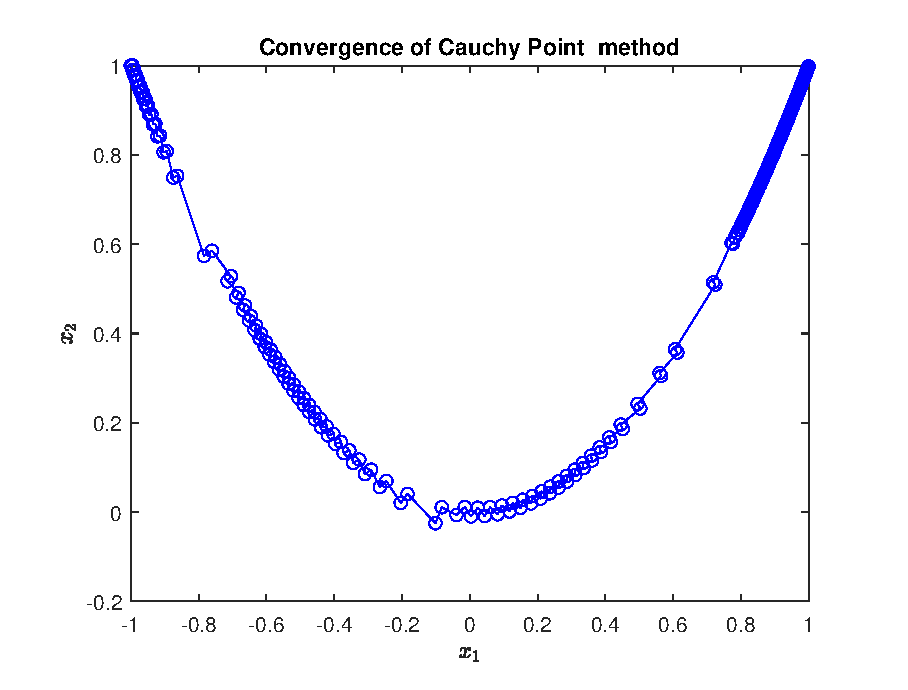
\includegraphics[width=\textwidth, trim={0cm 0cm 0cm 0cm}]{./figures/ex1-4-n1n1-cauchy-convergence.eps}
\end{figure}


\myFigureEnergy{Dogleg method}{ex1-4-n1n1-dogleg-energy}{ex1-4-n1n1-dogleg-energy.eps}
\begin{figure}[htbp]
\centering
\caption{Dogleg method convergence, $x_0 = \myvec{-1 \\ 1}$}
\label{ex1-4-n1n1-dogleg-convergence}
\includegraphics[width=\textwidth, trim={0cm 0cm 0cm 0cm}]{./figures/ex1-4-n1n1-dogleg-convergence.eps}
\end{figure}

\subsection*{5.}
Compare performance of the trust region based on Dogleg method for three different $\delta_0$. \\\newline

Argumented in previous answer 3.

\subsection*{6. (Bonus)}
Report the convergence history i.e., for each iteration, report the values of objective
function, trust-region-radius, and the ratio of the actual reduction to the predicted reduction.
(Please make a table.) \\\newline


Convergence history with $x_0 = \myvec{0 \\ 0}$ of objective function values 
comparing Cauchy Point and Dogleg methods: \\\newline

\begin{tabular}{|c|c|c|}
    \hline
    N & \textbf{Dogleg} & \textbf{Cauchy}  \\
    \hline
    1 & 1.0000 & 1 \\
    2 & 1.0000 & 1 \\
   3 & 0.7838 & 0.783752441406250 \\
    4 & 0.5165 & 0.667859425835307 \\
    5 & 0.3669 & 0.667859425835307 \\
    6 & 0.2193 & 0.611562564038043 \\
    7 & 0.1636 & 0.591324573691497 \\
    8 & 0.0621 & 0.573386256785240 \\
    9 & 0.0621 & 0.554558208423006 \\
    10 & 0.0398 & 0.537912629398300 \\
    11 & 0.0194 & 0.520195576039467 \\
    12 & 0.0044 & 0.504566856105441 \\
    13 & 0.0010 & 0.487682517002878 \\
    14 & 0.0000 & 0.472818613394980 \\
    15 & 0.0000 & 0.456491435839246 \\
    16 & 0.0000 & 0.442147412520641 \\
    \ldots & / & \ldots \\
    13972 & / & 7.8324e-13\\
    \hline
\end{tabular}



\end{document}
